% !TEX root = ../my-thesis.tex
%

\chapter{Ecological diversity within rear-edge: a case study from Mediterranean \Qpw}\label{sec:multivar}

\newpage

\paragraph{Abstract} \mbox{} \\
Understanding the ecology of populations located in the rear-edge of their distribution is key to assess the response of the species to changing environmental conditions. Here we focus on rear-edge populations of \Qpy in Sierra Nevada (southern Iberian Peninsula) to analyze their ecological and floristic diversity. We perform multivariate analyses using high-resolution environmental information and forest inventories to determine how environmental variables differ among oak populations, and to identify population groups based on environmental and floristic composition.
We find that water availability is a key variable in explaining the distribution of \Qp and the floristic diversity of their accompanying communities within its rear edge. Three cluster of oak populations were identified based on environmental variables. We found differences among these clusters regarding plant diversity, but no for forest attributes. A remarkable match between the populations clustering derived from analysis of environmental variables and the ordination of the populations according to species composition was found.
The diversity of ecological behaviors for \Qp populations in this rear edge are consistent with the high genetic diversity shown by populations of this oak in the Sierra Nevada. The identification of differences between oak populations within the rear-edge with respect to environmental variables can aid to plan the forest management and restoration actions, particularly considering the importance of some environmental factors in key ecological aspects.
\newpage

\section{Introduction}\label{sec:multivar:intro}

The study of ecological dynamics within the rear edge populations is considered essential to establish proper management guidelines under current climate uncertainties \autocite{Fadyetal2016EvolutionbasedApproach}. Rear-edge populations are often adapted to local environmental conditions at the limit of the species' ecological amplitude, and often show a long-term persistence \autocite{HampePetit2005ConservingBiodiversity}. Local responses to environmental changes may differ from the species mean response \autocite{Castroetal2004SeedlingEstablishment,Benavidesetal2013DirectIndirect,GeaIzquierdoCanellas2014LocalClimate,Matiasetal2017ContrastingGrowth}, and such differences may either promote or hamper the survival of edge populations under global change \autocite{BenitoGarzonetal2011IntraspecificVariability}. Furthermore, the heterogeneity in the response to climate change observed across ecological and geographical gradients \autocite{GeaIzquierdoetal2013GrowthProjections,Chenetal2015InfluenceClimate,DoradoLinanetal2019GeographicalAdaptation,PerezLuqueetal2020LanduseLegacies}, justifies the need to incorporate fine-scale variation of environment variables throughout species ranges to better understand species responses to global change \autocite{DeFrenneetal2013MicroclimateModerates,Oldfatheretal2020RangeEdges}. This is particularly important for mountain landscapes, where the topographic complexity may cause a decoupling between the climate and the geographic spaces \autocite{ElsenTingley2015GlobalMountain,Pirononetal2015GeographicClimatic}.

The environmental heterogeneity (microclimate, geomorphology, topography, etc.) found in mountains allows the existence of a diverse plethora of ecological conditions at very fine spatial scales \autocite{Hannahetal2014FinegrainModeling,KornerSpehn2019HumboldtianView}, offering an excellent opportunity to study ecological responses to future environmental changes \autocite{SpehnKorner2009MountainLaboratory,Kohleretal2014MountainsClimate,Payneetal2017OpportunitiesResearch,Zamoraetal2017GlobalChange}. Some tree species, such as \emph{Pinus sylvestris} and \emph{Quercus pyrenaica}, have their rear-edge populations located in mountainous areas of southern Europe. The topographic heterogeneity of such habitats, which act as microclimatic islands within a region of unsuitable climate for the persistence of these species, is likely to have a significant impact on persistence of these populations \autocite{MeineriHylander2017FinegrainLargedomain}. In these areas, the climate variation controlled by topography \autocite{Franklinetal2013ModelingPlant,Potteretal2013MicroclimaticChallenges} is hard to capture, and the fine scales non-climate factors (both biotic and abiotic) can be at least as much relevant for species distribution as climate \autocite{Loetal2010WordCaution} by modulating the direct effect of regional climate on individuals. Additionally, there are finer scale gradients nested within each mountain range, which reproduce rear, optimum and leading edge conditions making the interpretation of what is currently occurring in the so-called rear edge extremely complex \autocite{Benavidesetal2013DirectIndirect,Oldfatheretal2020RangeEdges}. When environmental conditions are homogeneous, similar responses are expected which facilitate future forecast. Conversely, if the environmental conditions are heterogeneous, we expect a variety of responses, which forces us to consider different future scenarios at a very fine spatial scale, since climate change sensitivities could strongly vary at local scales \autocite{Lindneretal2010ClimateChange,GeaIzquierdoCanellas2014LocalClimate,Titoetal2020MountainEcosystems}.

\Qpw (Pyrenean oak) is a deciduous Mediterranean tree species widely distributed throughout south-western France and the Iberian Peninsula reaching their southern limit in mountain areas of northern Morocco \autocite{Franco1990Quercus}. The rear-edge populations of this species are restricted to high-mountain areas where these populations persists as isolated nuclei with ecological conditions very different from those of the main distribution area. \Qp is considered one of the Mediterranean trees with a higher sensitivity to climate change \autocite{BenitoGarzonetal2008EffectsClimate,GarciaValdesetal2013ChasingMoving}. Several studies analyzed the potential effects of climate change on distribution of this species at different spatio-temporal scales \autocite{Benitoetal2011SimulatingPotential,BenitoGarzonetal2008EffectsClimate,BenitoGarzonetal2007PredictiveModelling,Felicisimo2011ImpactosVulnerabilidad,GeaIzquierdoetal2013GrowthProjections,RuizBenitoetal2013PatternsDrivers,RuizLabourdetteetal2013ChangesTree,Urbietaetal2011MediterraneanPine} forecasting a decrease in the suitable area of this tree species, particularly in its southern range.

Considering that the conservation strategies for tree species need to take into account the peculiarities of the rear-edge populations \autocite{HampePetit2005ConservingBiodiversity,Fadyetal2016EvolutionbasedApproach,Rehmetal2015LosingYour}, and the high vulnerability to climate change of \Qp \autocite{GarciaValdesetal2013ChasingMoving}, here we focus on the rear-edge populations of this species in the mountains of southern Iberian Peninsula to answer the question: Are the environmental conditions of the rear-edge populations of \Qp in Sierra Nevada homogeneous?. The answer to this question may be useful to analyze how the predicted climate changes would impact the rear-edge population, providing valuable information for the development of efficient forest management and restoration plans. We selected rear-edge populations of \Qp located in Sierra Nevada (Southern Iberian Peninsula), since peripheral forest tree populations located in mountain areas represent natural laboratories for resolving priority research questions \autocite{Fadyetal2016EvolutionbasedApproach}. Particularly, we hypothesize that the rear-edge populations of \Qp located in mountain areas are representative of different environmental conditions at local scale due to the strong topographic gradients available at the edge of its range. In this work we analyze whether these rear-edge populations inhabit similar environmental conditions. We also assess to what extent the environmental variability is matched by the floristic diversity of \Qp forests. Specifically, the objectives of the work were: \emph{(i)} to determine the most important environmental variables for the distribution of Pyrenean oak populations in Sierra Nevada; \emph{(ii)} to identify groups of Pyrenean oak populations based on floristic composition and environmental conditions; and \emph{(iii)} to unveil whether the rear-edge populations clustering according to environmental variables coincides with their grouping based on their floristic composition.

\section{Material and Methods}\label{sec:multivar:MatMet}
\subsection{Study area}\label{sec:multivar:StudyArea}
The study was conducted at the Sierra Nevada (Andalusia, SE Spain; \figref{fig:location-map}), a mountainous region covering more than 2000 km\textsuperscript{2} with an elevation range of between 860 and 3482 \emph{m.a.s.l.} The climate is Mediterranean, characterized by cold winters and hot summers, with a pronounced summer drought. The annual average temperature decreases in altitude from 12-16 ºC below 1500 \emph{m.a.s.l.} to 0 ºC above 3000 \emph{m.a.s.l.}. Annual precipitation ranges from less than 250 mm in the lowest areas of the mountain range to more than 700 mm in the highest peaks. Winter precipitation is mainly in the form of snow above 2000 \emph{m.a.s.l.}. Additionally, the complex orography causes strong climatic contrasts between south and north-facing slopes. This mountain range is considered one of the most important biodiversity hotspots in the Mediterranean region \autocite{Blancaetal1998ThreatenedVascular}, hosting 105 endemic plant species for a total of 2353 taxa of vascular plants (33\% and 20\% of Spanish and European flora, respectively) \autocite{Lorite2016UpdatedChecklist}. Forest cover in Sierra Nevada is dominated by pine plantations (\emph{Pinus halepensis} Mill., \emph{Pinus pinaster} Ait., \emph{Pinus nigra} Arnold subsp. \emph{salzmannii} (Dunal) Franco, and \emph{Pinus sylvestris} L.) covering approximately 37000 ha. Native forests are mainly dominated by holm oak (\emph{Quercus ilex} subsp. \emph{ballota} (Desf.) Samp.) occupying low and medium mountain areas (11000 ha.), and Pyrenean oak \emph{Quercus pyrenaica} Willd. ranging from 1100 to 2000 \emph{m.a.s.l.}, covering about 3000 ha \autocite{PerezLuqueetal2019MapEcosystems}.

\begin{figure}
	\centering
	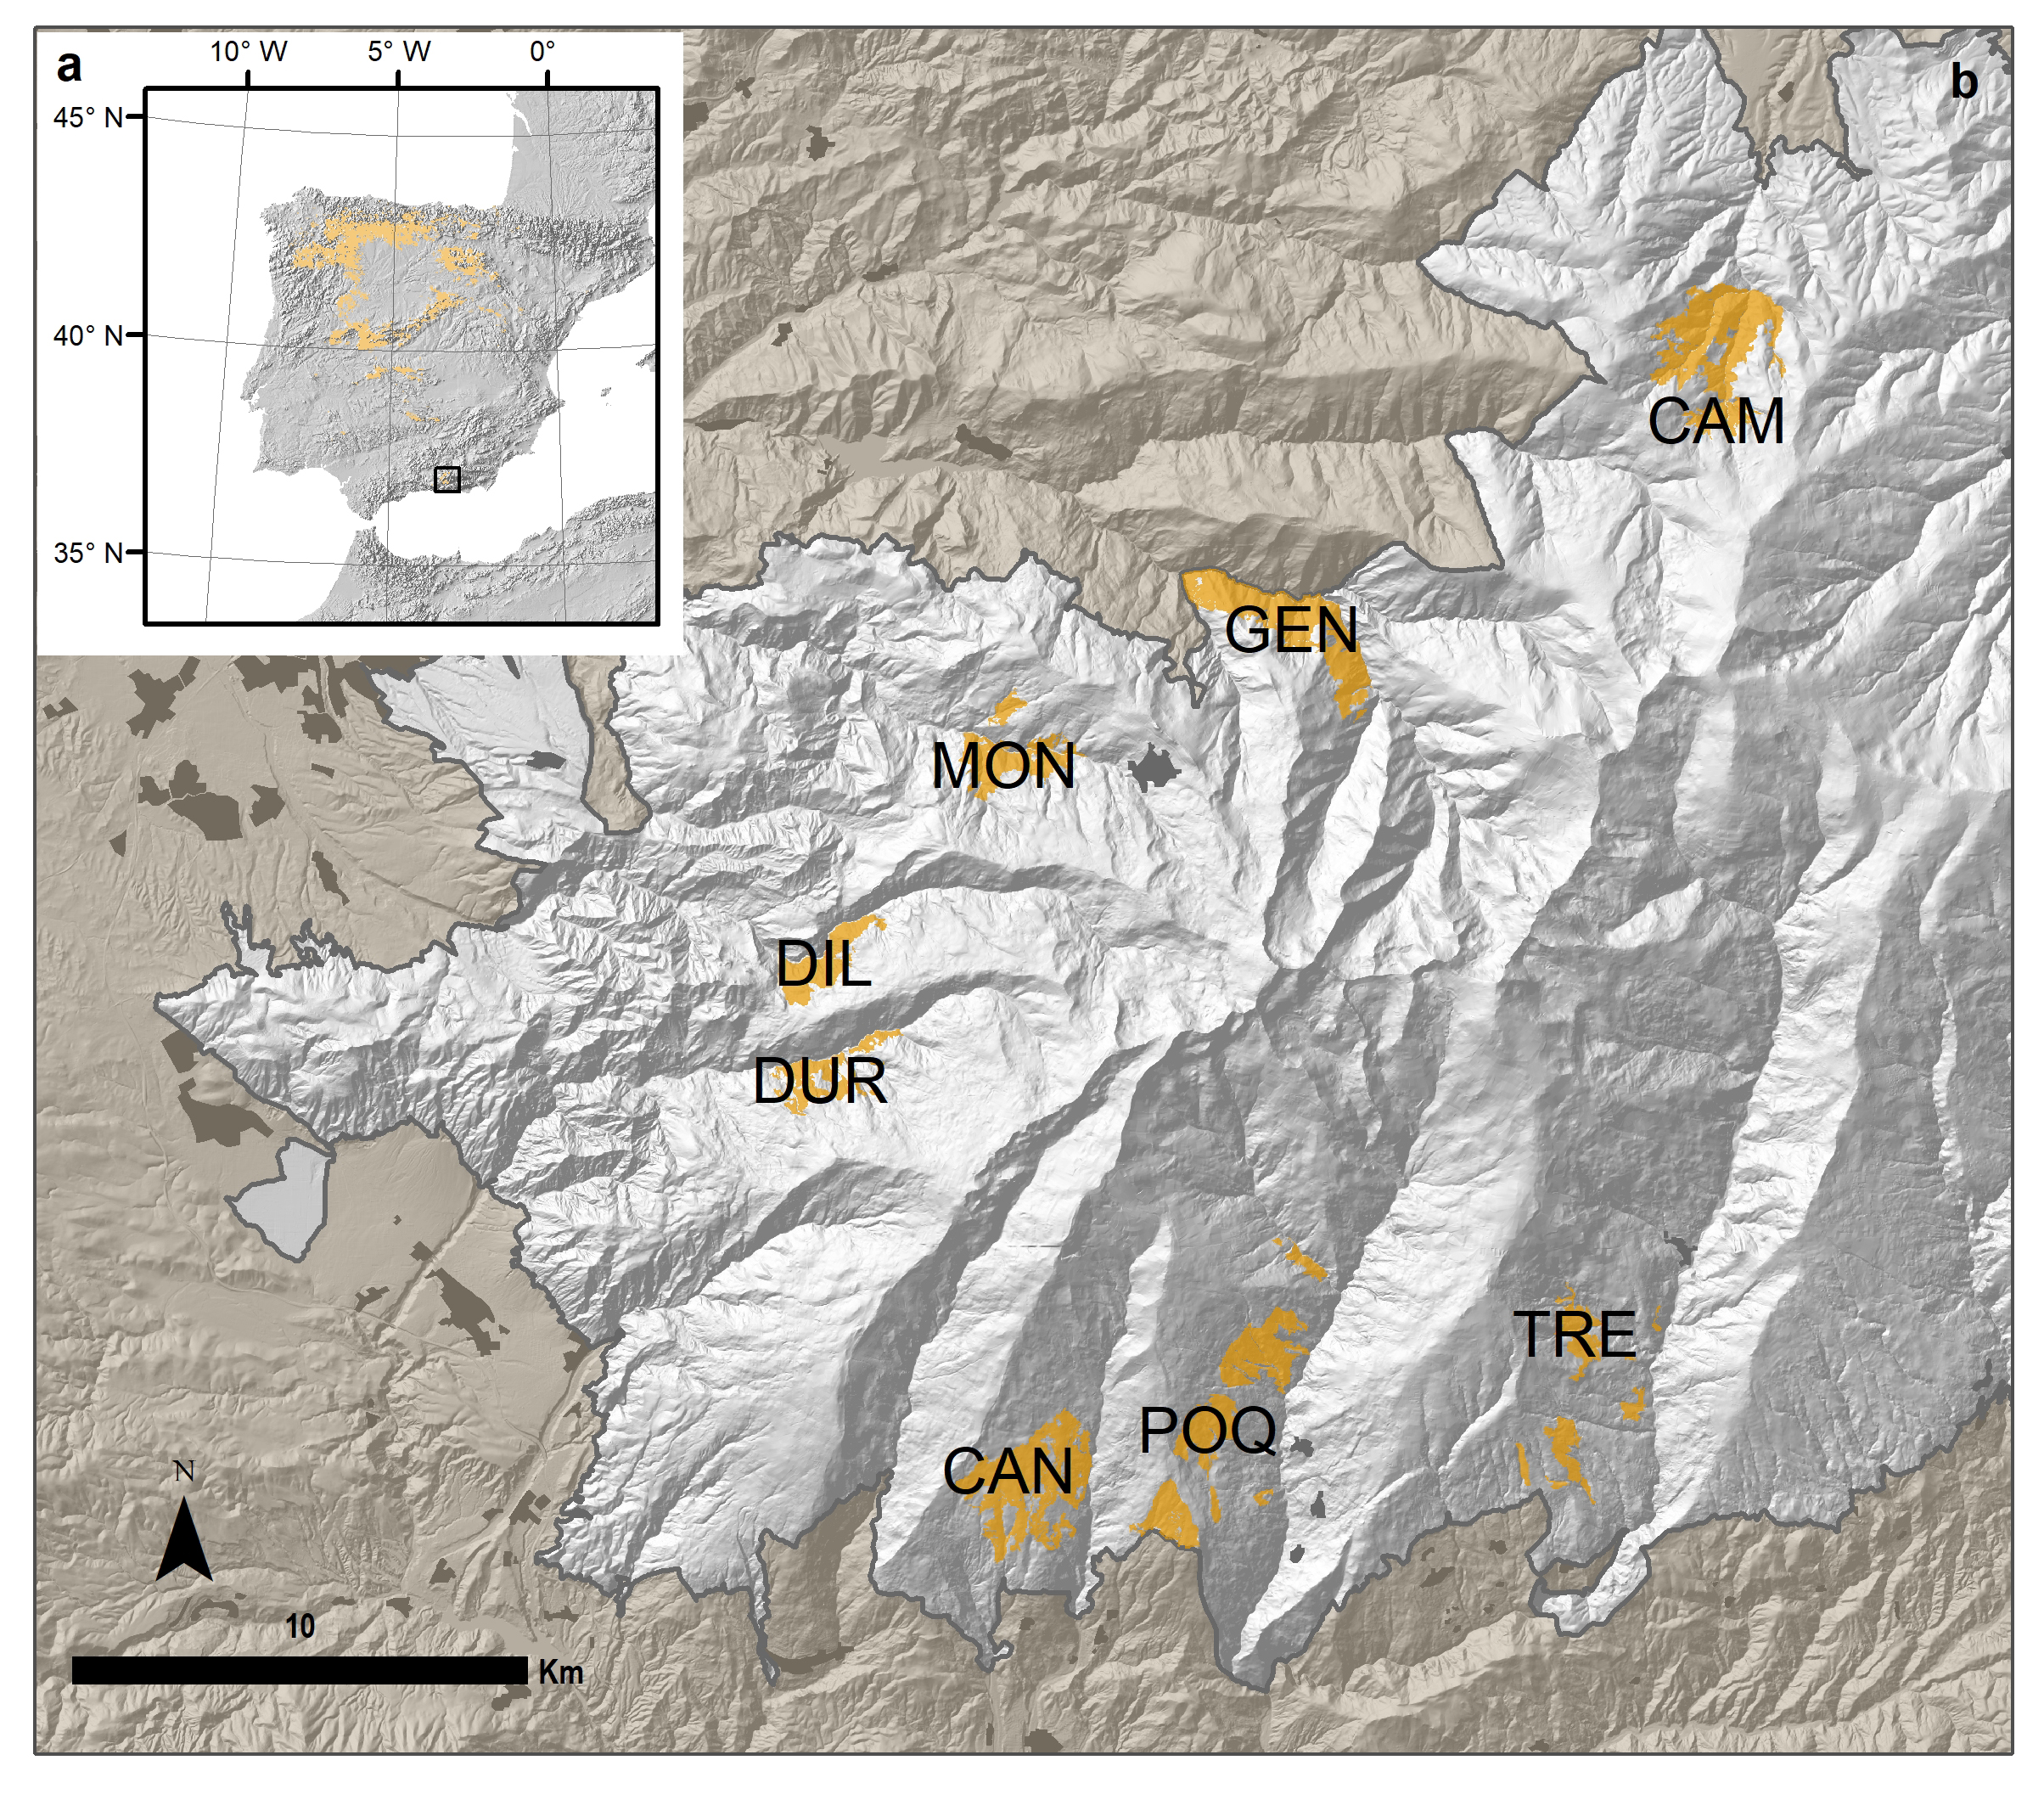
\includegraphics[width=\textwidth]{img/multivariante/dist_map_multivariante} \caption{Distribution of \textit{Quercus pyrenaica} forests in the Iberian Peninsula (\textbf{a}) and location of the patches in Sierra Nevada mountain range (\textbf{b}). Name of the each population as in \tabref{tab:tpop}.}\label{fig:location-map}
\end{figure}

\begin{sidewaystable} 
\caption{Description of the \Qp populations in Sierra Nevada. For elevation, minimum and maximum values are in brackets. The latitude and longitude coordinates referred to polygon centroid.}\label{tab:tpop}
\begin{adjustbox}{width=\linewidth}
	\begin{threeparttable}
		\begin{tabular}{@{}llllllll@{}}
			\toprule
			Oak poulation & Code & River valley & Municipalities & Elevation (m) & Latitude & Longitude & Area (ha) \\ \midrule
			El Camarate & CAM & Alhama & Lugros & 1740  (1441-2026) & 37º 10' 29.49'' N & 3º 15' 24.33'' W & 457.15 \\
			Robledal de San Juan & GEN & Genil & Güejar-Sierra & 1519  (1189-1899) & 37º 7' 29.63'' N & 3º 21' 54.60'' W & 395 \\
			Loma de la Perdíz & MON & Monachil & Monachil & 1780  (1564-1990) & 37º 5' 54.87'' N & 3º 25' 46.65'' W & 204.55 \\
			Umbría de la Dehesa de Dílar & DIL & Dílar & Dílar & 1764  (1478-1960) & 37º 3' 33.61'' N & 3º 28' 29.07'' W & 154.07 \\
			Loma de Enmedio & DUR & Dúrcal & Dúrcal & 1824  (1530-2035) & 37º 1' 58.75'' N & 3º 28' 38.44'' W & 137.04 \\
			El Robledal de Cáñar & CAN & Chico & Cáñar & 1687  (1366-1935) & 36º 57' 28.04'' N & 3º 25' 57.10'' W & 436.2 \\
			Loma de la Matanza y Loma de Ramón & POQ & Poqueira & Soportújar, Pampaneira, Bubión, Capileira & 1740  (1214-1981) & 36º 57' 58.90'' N & 3º 22' 55.12'' W & 458.95 \\
			Loma de los Lotes & TRE & Trevélez & Pórtugos, Busquístar & 1692  (1312-1963) & 36º 58' 37.38'' N & 3º 17' 25.75'' W & 197.92 \\ \bottomrule
		\end{tabular}
	\end{threeparttable}
\end{adjustbox}
\end{sidewaystable}

